\documentclass{article}
\usepackage{float}
% Language setting
% Replace `english' with e.g. `spanish' to change the document language
\usepackage[english]{babel}

% Set page size and margins
% Replace `letterpaper' with `a4paper' for UK/EU standard size
\usepackage[letterpaper,top=2cm,bottom=2cm,left=3cm,right=3cm,marginparwidth=1.75cm]{geometry}

% Useful packages
\usepackage{amsmath}
\usepackage{graphicx}
\usepackage[colorlinks=true, allcolors=blue]{hyperref}

\title{CrazyFlie}
\author{Thomas Evers and Noah Jadoenathmisier}

\begin{document}
\maketitle

\section{Introduction}
In this project, a Crazyflie drone was programmed to fly around a room while building a map of the room. A program that runs on a computer was made that allows a user to control the drone. From the interface of this program, the user can see the map of the room that the drone is creating. When the user clicks on a location on the map, the drone will automatically fly to the clicked location. The drone uses the RRT* pathfinding algorithm to find a path from its current location to the goal location without bumping into walls or obstacles. When the drone has not been to the goal location before, it will autonomously explore the room to find a path. If the drone sees new obstacles while flying, it will calculate a new route to the goal. The drone can also tell when obstacles have been removed. This means that the drone can deal with moving obstacles as well as stationary ones. When the drone is hovering in place it keeps detecting objects nearby. If an object gets too close, for example, a human who is walking in the room, the drone will avoid the object. Extra functions have been added. for example, manual control and drone spins. Special attention was given to reducing the calculation time needed for pathfinding.

\section{Hardware and API}
We used the Crazyflie drone for this project.
This is a small drone that comes with a Python library that allows you to control it.
Attached to the drone is a flow-deck.
This module uses a camera and the optical flow algorithm to track changes in the position of the drone.
On top of the drone, there is a range finder.
This allows the drone to detect the distance to the closest object in the 6 cardinal directions.

The drone connects to a laptop using the Crazy Radio.
This is a antenna that connects via USB to the laptop.
The Python API allows for reading the sensor values of the drone, as well as sending commands like "start going forward", or "turn 50 degrees to the left".

It has been observed that the flow-deck is very sensitive to the type of floor that the drone is flying over.
The best results seem to come from a floor with a lot of contrast and minimal reflections or specularity.

\section{GUI and Data Obtainment}
A GUI was created for the user to interface with the drones movement. One of the two main functions of the GUI was for the user to be able to input a desired location for the drone to manouver towards. The second function was to visualize the location of objects relative to the drone. The GUI will also show more detailed infomation about the drone. The GUI is shown below in Figure \ref{fig:GUI}.

\begin{figure}[H]
\centering
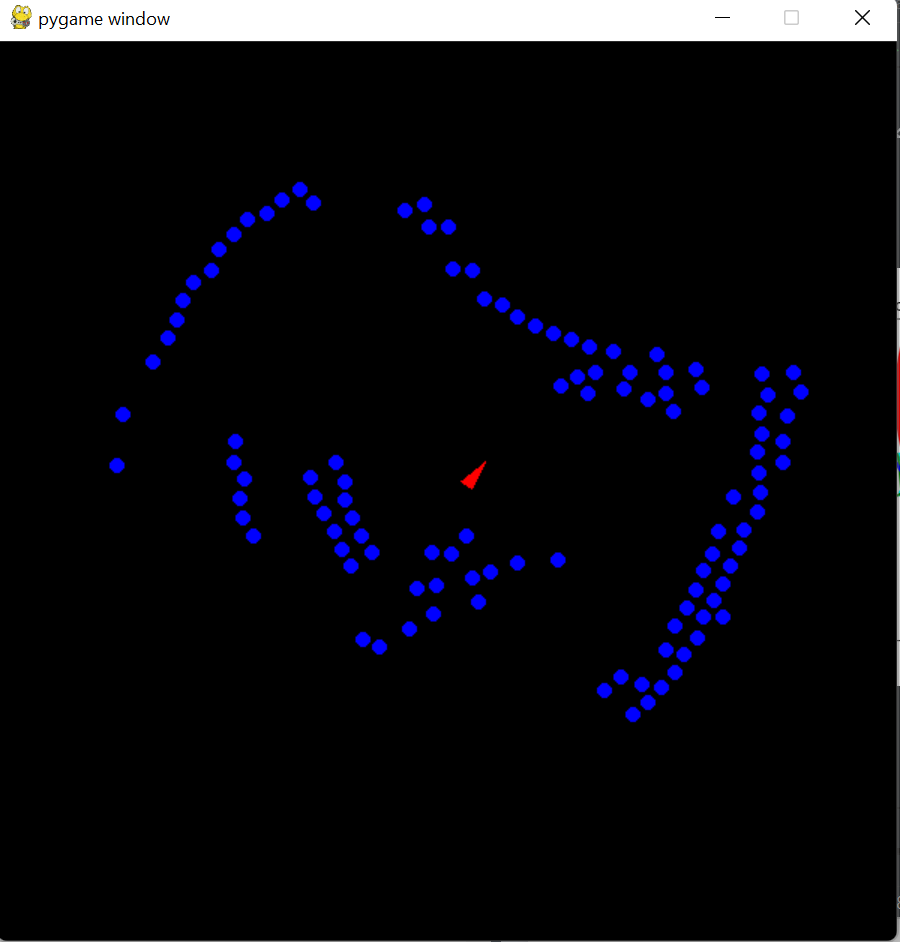
\includegraphics[width=0.6\textwidth]{PICS/Screenshot 2022-12-04 220849.png}
\caption{\label{fig:GUI}GUI showing drone with Obstacles}
\end{figure}

As can be seen the drone's location is shown on the GUI, as well as the locations of any objects. The locations of these objects were calculated by using information about the drones location and orientation in combination with distance measurements taken by the LIDAR sensors. In order to limit the amount of object data points pseudo duplicate measurements are ignored. The main reason for this is to optimize the path planning algorithm. Secondly, the drones actual location could shift relative to the estimation. The result of this would be that any previous measurement could be disagreed with by a current measurement. The previous measurement would be thrown out in this case seeing as current information is more valuable that past information. A way to use this past information instead of throwing it out would be to implement a SLAM algorithm. This is described in Section \ref{sec:SLAM}


\section{Path Planning}
\subsection{RRT*}
The path planning algorith that was implemented was RRT* , an adaptation of RRT(Rapidly exploding Random Tree). The RRT* algorithm is given a starting and end location, the locations of the objects and a distance from which the drone should stay away from all objects.

We have also implemented A* as a path-finding algorithm, but we decided to use RRT* because A* does not make full use of the drone's ability to move in all arbitrary directions.
Using the A* algorithm results in paths that contain many straight lines in cardinal and ordinal directions.

The RRT algorithm works by randomly adding nodes to a graph and connecting them to the nearest existing node. After a certain amount of iterations, a graph has been created and a discrete path planning algorithm such as Dijkstra's can be used to find the most optimal path in the graph from the start to the end node.
The RRT* algorithm is a version of the RRT algorithm that adds 2 rules. These 2 rules allow for the RRT* algorithm to create smoother paths, and be able to approach an optimal solution as the number of iterations goes to infinity.
The first rule is that when a random node gets added, instead of it being connected to the nearest existing node, it gets connected to any node within some radius that creates a shorter path.
The second rule, is that once this previous node is connected to another node creating a relatively low cost path. Any other nodes within some radius are checked, to see whether connecting them to the previous node decreases their path cost.

\begin{figure}[H]
\centering
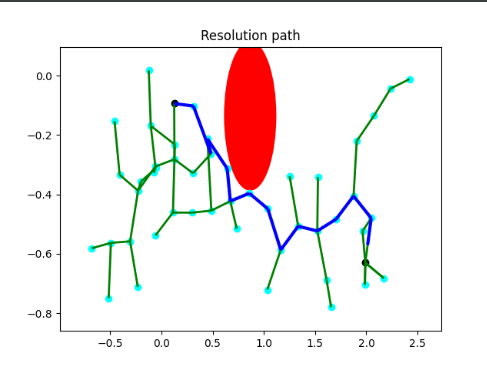
\includegraphics[width=0.6\textwidth]{PICS/path.png}
\caption{\label{fig:graph}Graph and path Created by the RRT* Algorithm}
\end{figure}

As can be seen in Figure \ref{fig:graph} the RRT algorithm creates a nice graph. After this Dijkstra's algorithm is used to find the lowest cost/fastest path within the graph.

This implementation of RRT* uses a 25 cm step size with a maximum of 200 iterations. In order to increase the computation time, a dynamic iteration limit was also set. It was set to double the amount of iterations after a valid path was found. For the example in Figure \ref{fig:graph} this decreased the iterations from 200 to 60, while still providing a more than valid path.

In later implementations optimisations were made making the maximum number of iterations and the step size variable based on factors such as object frequency and distance from start to finish.

\subsection{Path filtering}
After the RRT* algorithm is applied we are left with a decent path, but it is by no means optimal. One could increase the number of iterations to improve the quality of the path, but this would increase computation time, which is valuable, especially in more complex paths. One of the most important things we can do to increase the quality of the path taken, is to smooth it. A perfect amount of smoothing decreases the amount of unnecessary turns taken, but guarantees that no objects are hit taking shortcuts. For the implementation in this paper, the amount of nodes was artificially increased 5 fold, and then a 10 point moving average was applied. 
This led to the smooth path in Figure \ref{fig:smooth}

\begin{figure}[H]
\centering
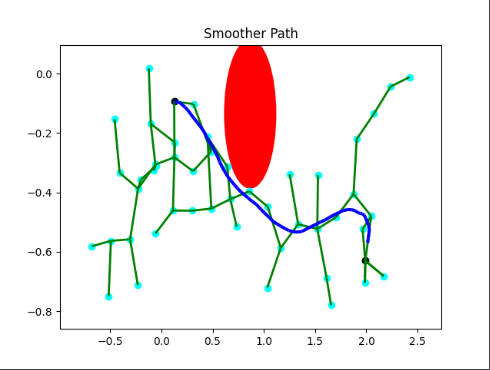
\includegraphics[width=0.6\textwidth]{PICS/smoothpath.png}
\caption{\label{fig:smooth}Smooth path Created by the RRT* Algorithm and a moving average}
\end{figure}

\section{Path following}
\subsection{How to follow path}
\paragraph{Constant Yaw}
When looking at how to implement the drone following the path described in Figure \ref{fig:smooth} there are several ideas that may come to mind. The first is to keep the yaw of the drone constant, this implies the drone faces the same direction during the flight. This would be implemented by telling the drone to move towards the next point in the path. When it reaches this point, it is removed from the path and the drone is told to go towards the next point in the path. This implementation is was implemented but led to problems with object detection. Seeing as the drone has 4 lidar sensors in the 2-d space being moved in, it can not see every object around the drone. Thus when moving at a 45 degree angle relative to the drone, it is very likely that it hits an object it never even saw coming. For this reason, this solution was not chosen.
\paragraph{Forward facing}
The next option was to always have the drone face the direction in which it is moving, this way any object in front of the drone will be detected and dealt with. This algorithm is implemented by having the drone move at a constant velocity forwards. Meanwhile the yaw rate is adjusted based on the error between the estimated yaw and angle required to face the next point in the path.
\paragraph{Constant Yaw-rate}
Another solution would be to have the drone fly down the path while having a constant yaw rate. The advantage of this would be that the drone would have constant access to all of the objects around it. This data could allow the drone to fly more optimally. However it was found during testing that a constant yaw rate significantly affected the location and yaw estimation of the drone. These inaccurate estimations had a more negative affect than the positive affect of a constant yaw rate. 
Because of this the forward facing solution was implemented. The GUI showing this situation can be seen in Figure \ref{fig:pathExecute} below.
\begin{figure}
\centering
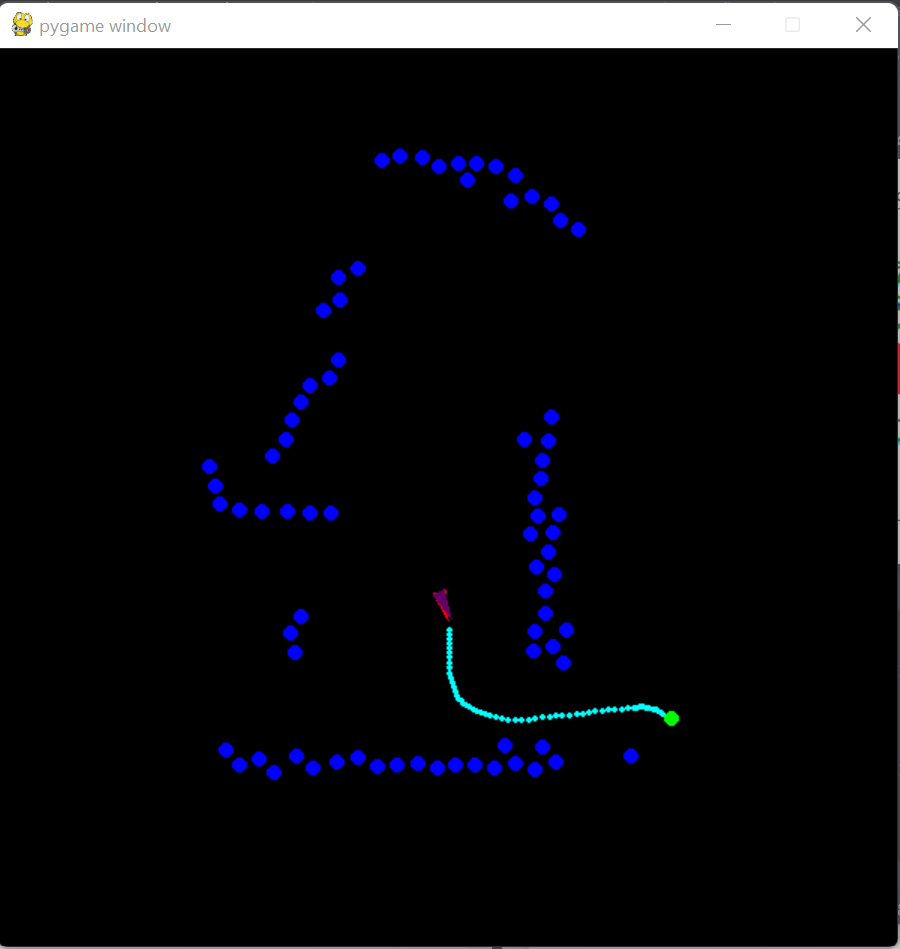
\includegraphics[width=0.6\textwidth]{PICS/DecentPathCreation.png}
\caption{\label{fig:pathExecute}Path Created and Followed by the Drone shown in GUI}
\end{figure}


\subsection{Object Detection}
An important aspect, if not the most important aspect of software that allows a drone to find its way through an obstacle field, is for the drone to avoid obstacles. Originally the drone may follow a path assuming very little obstacles based on its few measurements. The drone will fly until it measures an obstacle in its path. The implementation in this paper deals with that in the following way. If there is a single obstacle within some range of it, it moves away from the obstacle. If there are multiple objects in its proximity, it calculates a weighted center of these obstacles, where a closer obstacle is weighted higher. The drone will then fly away from the center of these obstacles. Once it deems itself in a safe location, it scans its entire surroundings properly and then recalculates a path. It then repeats the entire process until it reaches its destination.


\section{Future Improvements}
\subsection{SLAM / data mapping}
\label{sec:SLAM}
A SLAM algorithm, or Simultaneous Localisation and Mapping algorithm, locates and maps at the same time, as the name suggests. In the current version, it is assumed that the drones state estimation is perfect when taking the measurements. This is certainly not the case. The drone shifts quite a lot from its estimated location over time. This causes measurements from 5 seconds ago to be less accurate. And measurements from 20 seconds ago to be useless. SLAM algorithms are a way of improving the accuracy and validity of past measurements. They are also a way to improve the drones current state estimation based on these measurements.
A SLAM algorithm has not been implemented but its advantages are noteworthy.

\subsection{Exploration}
In order to make the drone map out an entire room, the first thing that is required is that past measurements can be accurately linked to current measurements. For this a SLAM algorithm is required. Assuming a SLAM algorithm, a exploration mode can be designed, in which the drone is tasked to attempt to reach random points it has not been to in a designated square. This way soon it will map out the entire room.




\bibliographystyle{alpha}
\bibliography{sample}

\end{document}
